\documentclass[9pt]{article}
\usepackage{fullpage,amsmath,url,cases}
\usepackage{natbib,longtable,graphicx,tikz}
%\usepackage{subfig}
\usepackage{url}
\usepackage{pdfpages}
\usepackage{hyperref, natbib}
%\@ifundefined{showcaptionsetup}{}{%
%\PassOptionsToPackage{caption=false}{subfig}}
\graphicspath{{./figures/}{./figures/otherFigures/}}
\usepackage{xcolor}
\usepackage{colortbl}
\definecolor{RubineRed}{RGB}{240, 0, 240}       % RubineRed  Approximate PANTONE RUBINE-RED
%\usepackage{subfig}
\usepackage{listings}
\usepackage{color}

%%%%%%%%%%%%%%%%%%%%%%%%%%%%%%%%%% referencing %%%%%%%%%%%%%%%%%%%%%%%%%%%%%%%%%%
\usepackage{natbib}
\usepackage{hyperref}
\usepackage{xcolor}
\hypersetup{
    colorlinks,
    %linkcolor={red!50!black},
    linkcolor={black},
    citecolor={blue!50!black},
    urlcolor={blue!80!black}
}

%%%%%%%%%%%%%%%%%%%%%%%%%%%%%%%%%%%%%%%%%%%%%%%%%%%%%%%%%%%%%%%%%%%%%%%%%%%%%%%%
\usepackage[disable]{todonotes}

\usepackage{placeins}
\usepackage{flafter}

\newcounter{todocounter}
\newcommand{\todonum}[2][]
{\stepcounter{todocounter}\todo[#1]{\thetodocounter: #2}}

\newcommand{\done}[2][]
{\todo[color=green!40, #1]{#2}}

\newcommand{\donenum}[2][]
{\stepcounter{todocounter}\done[#1]{\thetodocounter: #2}}
%%%%%%%%%%%%%%%%%%%%%%%%%%%%%%%%%%%%%%%%%%%%%%%%%%%%%%%%%%%%%%%%%%%%%%%%%%%%%%%%

\definecolor{dkgreen}{rgb}{0,0.6,0}
\definecolor{gray}{rgb}{0.5,0.5,0.5}
\definecolor{mauve}{rgb}{0.58,0,0.82}

\lstset{frame=tb,
  language=Java,
  aboveskip=3mm,
  belowskip=3mm,
  showstringspaces=false,
  columns=flexible,
  basicstyle={\small\ttfamily},
  numbers=none,
  numberstyle=\tiny\color{gray},
  keywordstyle=\color{blue},
  commentstyle=\color{dkgreen},
  stringstyle=\color{mauve},
  breaklines=true,
  breakatwhitespace=true,
  tabsize=3
}
\lstset{language=bash}


\title{Supplementary Material}
\author{Sha Joe Zhu, Jacob Almagro-Garcia, Jason Hendry and Gil McVean}
\date{}

\usepackage[label font=bf,labelformat=simple, position = top, justification=RaggedRight,singlelinecheck=false]{subfig}
\renewcommand{\thesubfigure}{\Alph{subfigure}}

\setcounter{equation}{0}
\setcounter{figure}{0}
\setcounter{table}{0}
\setcounter{page}{1}
\makeatletter
\renewcommand{\thesection}{S\arabic{section}}
\renewcommand{\theequation}{S\arabic{section}.\arabic{equation}}
\renewcommand{\thefigure}{S\arabic{section}.\arabic{figure}}
\renewcommand{\thetable}{S\arabic{section}.\arabic{table}}
\renewcommand{\bibnumfmt}[1]{[S1#1]}
\renewcommand{\citenumfont}[1]{S1#1}
%%%%%%%%%% Prefix a "S" to all equations, figures, tables and reset the counter %%%%%%%%%%

%\floatsetup[figure]{style=plain,subcapbesideposition=top}
%\newsubfloat{figure}



%%%%%%% Start on new page
\renewcommand{\thepage}{S1-\arabic{page}}
\begin{document}
\listoftodos
\clearpage
%\setcounter{page}{1}

\maketitle
\tableofcontents

%\setcounter{section}{0}

\newpage

\section{Deconvolution in the presence of IBD}
\subsection{Notations}
We use the same notations as \citet{Zhu2017} (see Table~\ref{tab:notation}). Our data, $D$, are the allele read counts of sample $j$ at a given site $i$, denoted as $r_{j,i}$ and $a_{j,i}$ for reference (REF) and alternative (ALT) alleles respectively.  These have assigned values of $0$ and $1$, respectively. Here we consider only bi-allelic loci, though future extensions to the model to include multi-allelic sites could be accommodated.  The empirical allele frequencies within a sample (WSAF) $p_{j,i}$ and at population level (PLAF) $f_i$ are calculated by $ \frac{a_{j,i}}{a_{j,i} + r_{j,i}}$ and $ \frac{\sum_j a_{j,i}}{\sum_j a_{j,i} + \sum_j r_{j,i}}$ respectively. Since all data in this section refers to the same sample, we drop the subscript $j$ from now on.

\begin{table}[htb]\centering
\begin{tabular}{c|c}\hline
$i$              & Marker index\\
$j$              & Sample index \\
$r$              & Read count for reference allele \\
$a$              & Read count for alternative allele \\
$f$              & Population level allele frequency (PLAF) \\
$n$              & Number of strains within sample \\
$l$              & Sequence length \\
$\mathbf{w}$      & Proportions of strains \\
%$\mathbf{x}$	& Log titre of strains \\
$\mathbf{h}_{i}$ & Allelic states of $n$ parasite strains at site $i$ \\
$h_{k,i}$   & Allelic state of parasite strain $k$ at site $i$\\
$p$              & Observed within sample allele frequency (WSAF) \\
$q$              & Unadjusted expected WSAF  \\
$\pi$            & Adjusted expected WSAF \\
%$\Xi$            & Reference panel\\
%$\xi_{k,i}$     & Allelic state of reference panel strain $k$ at site $i$\\
%$G$              & Scaling factor used for genetic map\\
$e$              & Probability of read error\\
$\mathcal{S}_{i}$ & IBD state at site $i$ \\
$\mathcal{G}$ & Genotype state at site $i$ \\
\hline
\end{tabular}
\vspace{.2cm}
\caption{Table summarising the notation used in this article.}\label{tab:notation}
\end{table}

\subsection{Modelling with IBD state}
We describe the mixed infection problem by considering the number of strains, $n$, the relative abundance of each strain, $\mathbf{w}$, and their allelic states, $\mathbf{h}_{i}$. In addition to \citet{Zhu2017}, we also infer the IBD-state $\mathcal{S}_{i}$, which describes the strain relationship with each other at each site $i$. For example, for three strains, the IBD-state could be one of the five cases: (1) all strains are not IBD; (2)(3)(4) only two strains are IBD; (5) all strains are IBD (see Table~\ref{tab:encode}). To simplify our problem, we assume independence between each marker, and drop the subscript $i$ from now on. Similar to \citet{Jack2016}, we use a Bayesian approach and define the posterior probabilities of $n$, $\mathbf{w}$, $\mathbf{h}$ and $\mathcal{S}$,  as:

\begin{equation}
P(n, \mathbf{w}, \mathbf{h}, \mathcal{S}| e, D) \propto L(n, \mathbf{w}, \mathbf{h}, \mathcal{S} | e, D) \times P(n, \mathbf{w}, \mathbf{h}, \mathcal{S}), \label{eqn:post}
\end{equation}
where $e$ is the read error rate.

\begin{table}{h}
\centering
\begin{tabular}{c|ccc}
  Index / & \multicolumn{3}{c}{IBD state} \\
viterbi state    & k = 2& k = 3 & k = 4 \\ \hline
1	  &1-2	&	1-2-3	&1-2-3-4	\\
2	  &2-2	&	2-2-3	&2-2-3-4	\\
3	  &	  	&	3-2-3	&3-2-3-4	\\
4	  &		  &	1-3-3	&4-2-3-4	\\
5	  &		  &	3-3-3	&1-3-3-4	\\
6	  &	  	&		    &3-3-3-4	\\
7	  &	  	&		    &4-3-3-4	\\
8	  &	  	&	    	&1-4-3-4	\\
9	  &	  	&		    &4-4-3-4	\\
10	&	  	&		    &3-4-3-4	\\
11	&	  	&		    &1-2-4-4	\\
12	&		  &		    &2-2-4-4	\\
13	&	  	&		    &4-2-4-4	\\
14	&	  	&	    	&1-4-4-4	\\
15	&	  	&		    &4-4-4-4	\\
\end{tabular}
\caption{IBD configurations of number of strains are 2, 3 and 4. The state 1-2 denotes that strains 1 and 2 are non-IBD; The state 2-2 denotes that strain 1 is IBD with strain 2. The state 2-2-3 denotes that strain 1 is IBD with strain 2, but not strain 3. }\label{tab:encode}
\end{table}


\noindent We assume a prior in which the haplotypes of the $n$ strains are independent of each other and dependent only on the IBD state. Let $\mathcal{G}$ be the genotype state that is derived from the IBD state $\mathcal{S}$. We assume uniform prior on $\mathcal{G}|\mathcal{S}$. For example, if $n=3$ and only strains 1 and 2 are IBD, the genotype state at site $i$ $\mathcal{G}$ could be $\{0,0,0\}$; $\{0,0,1\}$; $\{1,1,0\}$ and $\{1,1,1\}$. Therefore, we can decompose the joint prior as:
\begin{equation}
P(n, \mathbf{w}, \mathbf{h}, \mathcal{S}) = P(n) \times P(\mathbf{w}|n) \times P(\mathbf{h} , \mathcal{S}|n),
\end{equation}
where
\begin{equation}
P(\mathbf{h}, \mathcal{S}|n) = P(\mathcal{S}|n) \times \sum_{\xi \in \mathcal{G}} P(\mathbf{h} | \xi) \times P(\xi|\mathcal{S}).
\label{eqn:ibd_prior}
\end{equation}

\noindent For details of the likelihood and the prior on the proportions see \citet{Zhu2017} sections 2.2.1 and 2.2.2. We use the following expression for the expected WSAF $q$, as:
\begin{equation}
q = \mathbf{w}\cdot\mathbf{h}.\label{eqn:qij_full_sum}
\end{equation}



\noindent The data, which can be summarised by the reference and alternative allele read counts at each site, is modelled through a beta-binomial distribution given the expected WSAF.  We model the data at distinct segregating sites as independent.  Thus the likelihood function  in Eqn.~\eqref{eqn:post} is only dependent on the haplotypes  and their frequencies through their contribution to $q_{i}$.

%; i.e. $L(n, \mathbf{w}, \mathbf{h}, | \Xi, e, D) = \prod_{i=1}^l L(q_i | \Xi, e, D)$.

To incorporate sequencing error, we modify the expected WSAF such that the allele frequency of `REF' reads as `ALT' is $(1 - q_i)e$, and the allele frequency of `ALT' reads as `REF' is $q_ie$. Thus, the adjusted expected WSAF becomes:

\begin{equation}
\pi_i = q_i + (1 - q_i)e - q_ie = q_i + (1 - 2q_i)e.\label{eqn:adj_q}
\end{equation}

\noindent We model over-dispersion in read counts relative to the Binomial using a Beta-binomial distribution. Please see {\bf Technical details} for likelihood calculations.

\subsection{Technical details}

To infer the relatedness between strains within in a mixed infection and their relative proportions we use a Markov chain Monte Carlo (MCMC) approach. We learn the relative abundance of each strain by exploiting signatures of within-sample allele frequency imbalance, using a Metropolis-Hastings algorithm, which samples proportions ($w$) given IBD-configurations ($\mathcal{S}$). We then use a Gibbs sampler to update $\mathcal{S}$ for a given $w$ by sampling the IBD state from the posterior, and sample the genotype from the selected IBD state to update haplotypes.

\donenum{Sup. Mat. 2, describe the model in more detail}
\donenum{Sup. Mat. 6, Description of MCMC for IBD inference}
\subsubsection{Metropolis-Hastings update for proportions}\label{sec:updateP}
We update $\mathbf{w}|n$, through the underlying log titres, $\mathbf{x}|n$. Specifically, we choose $i$ uniformly from $n$ and propose new $x_i'$s from $x_i' = x_i + \delta x$, where $\delta x \sim N(0, \sigma^2/s)$, and $s$ is a scaling factor. The new proposed proportion is therefore $\frac{\exp(x_k')}{\sum_{k=1}^n \exp(x_k')}$. Since the proposal distribution is symmetrical, the Hastings ratio is 1. A new update is accepted with probability

 $$\min\left(1, \frac{P(\mathbf{w}'|n)}{P(\mathbf{w}|n)} \frac{L(\mathbf{w}', \mathbf{h}, {\mathcal S} | e, D)}{L(\mathbf{w}, \mathbf{h}, {\mathcal S} | e, D)}\right).$$

\subsubsection{Gibbs sampling for haplotype and IBD-configuration update}
\donenum{Major 7: What does this mean, and why did the new method perform more poorly than the original}
In the new method, {\tt DEploidIBD} does not reinforce any haplotype structure. At every site, the posterior probability maximizes at IBD state. We use a two-layer hidden markov model framework to define our prior on IBD-configuration and haplotypes (Equation~\eqref{eqn:ibd_prior}). At the top layer, we have transitions between IBD-states, which reflect recombination events. From the top layer to the second layer, we defined a shrinkage prior, which computes the effective number of strains, and generate a binomial distribution for number of unique haplotypes given the probability of $\theta$, which is a beta random variable with shape parameters of effective number of strains ($K_{e}$) and difference between max number of strains and $K_{e}$. This genotype prior inclines to merge haplotypes to enable inbreeding. At the second layer, we make $P(\mathbf{h} | \xi) = 1$, and strictly copy the underline genotypes (from the IBD state) as the allelic state. The impact of sequencing error on the expected WSAF is adjusted using equation \eqref{eqn:adj_q}.
\donenum{Sup. Mat. 3, what is meant by “genotypes” vs. “alleles”}

\vspace{.2cm}

\noindent{\bf Caveat: identifiability with balanced mixing}\\
Using a reference panel free approach means that it can be difficult to deconvolve samples containing strains with equal proportions. For example, without a reference panel, we assume independence between loci, and it is difficult to distinguish between $\{\frac{1}{3},\frac{1}{3},\frac{1}{3}\}$ and $\{\frac{1}{3},\frac{2}{3}\}$, or
$\{\frac{1}{4},\frac{1}{4}, \frac{1}{4}, \frac{1}{4}\}$ and $\{\frac{1}{4},\frac{1}{4}, \frac{1}{2}\}$, or $\{\frac{1}{5},\frac{1}{5}, \frac{1}{5}, \frac{1}{5}, \frac{1}{5}\}$ and $\{\frac{1}{5},\frac{1}{5}, \frac{3}{5}\}$, $\{\frac{1}{5},\frac{2}{5}, \frac{2}{5}\}$ and
$\{\frac{1}{5},\frac{1}{5}, \frac{1}{5}, \frac{2}{5}\}$. We advise users to apply {\tt DEploid} with multiple runs with and without the `-ibd' flag and see if such problem occurs.


%Pf3D7\_01\_v3	&	95754	&	0	&	0	&	1	&	0	\\
%Pf3D7\_01\_v3	&	100330	&	0	&	1	&	0	&	0	\\

%\begin{center}
  %\begin{tabular}{cccccc}
    %CHROM	&	POS	&	3D7	&	Dd2	&	HB3	&	7G8	\\
%Pf3D7\_01\_v3	&	94487	&	0	&	0	&	0	&	1	\\
%Pf3D7\_01\_v3	&	95518	&	0	&	1	&	1	&	0	\\
%Pf3D7\_01\_v3	&	95632	&	0	&	0	&	1	&	0	\\
%Pf3D7\_01\_v3	&	95641	&	0	&	0	&	1	&	0	\\
%Pf3D7\_01\_v3	&	95680	&	0	&	0	&	1	&	0	\\
%Pf3D7\_01\_v3	&	95685	&	0	&	0	&	1	&	0	\\
%Pf3D7\_01\_v3	&	95686	&	0	&	0	&	1	&	0	\\
%Pf3D7\_01\_v3	&	95754	&	0	&	0	&	1	&	0	\\
%Pf3D7\_01\_v3	&	100330	&	0	&	1	&	0	&	0	\\
%Pf3D7\_01\_v3	&	100608	&	0	&	1	&	0	&	1	\\
%Pf3D7\_01\_v3	&	101269	&	0	&	1	&	1	&	1	\\
  %\end{tabular}
%\end{center}





\subsection{Implementation details}
\begin{itemize}
%We then compute the likelihood as $\frac{x^{\alpha-1}(1-x)^{\beta-1}} {\Beta(\alpha,\beta)}\!$, where

%${\displaystyle \mathrm {B} (\alpha ,\beta )={\frac {\Gamma (\alpha )\Gamma (\beta )}{\Gamma (\alpha +\beta )}}}$

\item {\bf Likelihood surface}
In the new version {\tt DEploidIBD}, the likelihood for WSAF is computed accordingly to the changes in the previous step. In principle, it is still in for form of
\begin{equation}
L(q_{i}| e, D) \propto \frac{\Gamma(a_i + \alpha) \Gamma(r_i + \beta)}{\Gamma(\alpha)\Gamma(\beta)}. \label{eqn:llk}
\end{equation}

For the first part of the {\tt DEploidIBD}, instead of computing the likelihood of a given WASF, we integrate the likelihood over the possible span of WSAF values.. Given the integrated likelihood surface, we compute the likelihood for WSAF = 0 and WSAF = 1. We use these two values as shape parameters of a beta distribution, $\alpha = llk_{0}$ and $\beta = llk_{1}$.

For the second part of {\tt DEploidIBD} inferring haplotypes from a given reference panel, the likelihood in Equation~\ref{eqn:llk} is computed the same as \cite{Zhu2017}. Specifically, the read counts of `ALT' are identically and independently distributed (i.i.d.) Bernoulli random variables with probability of success $v_i$; i.e. $a_i \sim Binom(a_i + r_i, v_i)$, and $v_i \sim Beta(\alpha, \beta)$, where $E(v_i) = \alpha/(\alpha+\beta) = \pi_{i}$. This is achieved by setting $\alpha = c\cdot \pi_{i} $ and $\beta = c\cdot (1-\pi_{i})$, such that the variance of the WSAF is inversely proportional to $c$. \textcolor{black}{The parameter $c$ (Equation~\eqref{eqn:llk}) reflects how much data are available. The mean coverage of the validation data set ranges from 106.20 to 147.04, with a mean of 124.487.} In practice, we set the parameters $c=100$.

%ibd state configuration, haplotype state configuration.

\item {\bf MCMC parameters for deconvolution}

\begin{itemize}
\item {\bf Number of strains}. As described above, we aim to infer more strains than are actually present, starting the MCMC chain with a fixed $n$, which has a default of $5$. \textcolor{red}{In our experience, we use the flag {\tt -k} to specify the number of strains as 4.} At the point of reporting, we keep strains with a proportion above a fixed threshold, typically $0.01$.

\item {\bf Parameters}. In practice, we set the parameters $\eta = 0$, \textcolor{black}{$\sigma^2 = 5$ which are adjusted accordingly when working with extremely unbalanced samples (see \citet{Zhu2017} supplementary material)}.  We set the read error rate as 0.01 and the rate of mis-copying as 0.01.

\item {\bf Recombination rate and scaling}. We assume a uniform recombination map, where the genetic distance between loci $i$ and $i+1$ is computed by $\psi_i = D_i / d_m$ where $D_i$ denotes the physical distance between loci $i$ and $i+1$ in nucleotides and $d_m$ denotes the average recombination rate in Morgans bp$^{-1}$. We use the recombination rate for {\it P. falciparum} of 13,500 base pairs per centiMorgan as reported by \citet{Miles2016}. \donenum{Minor Comment 6, on the scaling parameter G }The recombination rate is scaled by a factor $G$, which reflects the effective population size, rate of inbreeding, and relatedness of the reference panel. \textcolor{red}{In practice, we deconvolve over 1 million markers in field samples. We tune the parameter $G$ using {\it in vitro} lab mixtures, use a value of $G=20$ to ensure small values for recombination probabilities between any two markers, with a mean of 0.015. A large value of $G$ relaxes the reference panel constraint, becoming an LD free model when $G$ is infinity. The scaled genetic distance $G\psi$ is used to compute the transition probability of switching from copying reference haplotype $a$ to reference haplotype $b$. Given LD varies enormously between {\it P. falciparum} populations, we will investigate how to tune this parameter for future improvement. In the current release, our program allows users to apply the flag {\tt -G} and specify an input parameter $G$.} %For IBD track computation, we set $G = 0.1$ to enforce less recombination.

\item {\bf IBD state transitions} A significant improvement from \citet{Zhu2017}'s method is that $P(\mathcal{S}_{i}|n)$ takes into account of the IBD state at the previous position $i-1$ with recombination. A transition into a different IBD state will take into account of recombination probabilities.

\item {\bf Update without linkage disequilibrium}. For initialising the chain, or if the markers present are very widely spaced, linkage disequilibrium can be ignored, which is equivalent to setting the genetic distance between adjacent loci to be infinitely high.  Under these circumstances, the haplotype updates become much simpler and depend only on the population-level allele frequency (PLAF), for example as estimated from the reference panel or provided independently.

\item {\bf Reporting} We aim to provide users with a single point estimate of the haplotypes and their proportions, although the full chain is also available for analysis.  To achieve this we report values at the last iteration - i.e. we report a single sample from the posterior.  However, to measure robustness, we typically repeat the deconvolution with multiple random starting points\textcolor{black}{. We use a majority vote rule on the inferred number of strains; we then select the chain with the lowest average deviance (after removing the burn-in) as our estimate. The deviance measures the difference in log likelihood between the fitted and saturated models, the latter being inferred by setting the WSAF to that of the observed values.} These parameters can be modified by users to achieve a preferred balance between computational speed and confidence.  By default, we set the MCMC sampling rate as 5, with the first 50\% of samples removed as burn in and 800 samples used for estimation.

\item {\bf Reference panel construction}. To infer clonal samples for the reference panel we use the Pf3k project data, running the algorithm without LD on all samples and identifying those with a dominant haplotype (proportion $>$ 0.99) as clonal.  These clonal samples are grouped by region of sampling to form location-specific reference panels.  In addition, we have included a number of reference strains, described in more detail below.

\end{itemize}


  %\item {\bf Extract crossover events} We treat genome regions of which IBD posterior probabilities greater than 90\% as IBD blocks. Regions that are not identified by a particular IBD region are crossover event candidates. We identify the candidate region of which two sides belong to different IBD blocks as a crossover event.

%\item {\bf MCMC parameters for recombination map and smoothing}
%We burn the first 10\% of the MCMC chain, and draw every 5th sample of the chain. To collect 1000 samples for each SNP interval.
\end{itemize}




\subsection{Commands}
Each isolate deconvolution is repeated 15 times with a random seeds of choice from 1 to 15. We take the seed with the smallest value such that the number of strain is the consensus one.
\linespread{1}
\begin{lstlisting}
ref=PD0577-C_ref.txt
alt=PD0577-C_alt.txt
plaf=asiaGroup1_PLAF.txt
panel=asiaGroup1PanelMostDiverse10.csv
exludeAt=asiaGroup1_and_pf3k_bad_snp_in_at_least_50_samples.txt

prefix=PD0577-C_IBD
time dEploid -ref ${ref} -alt ${alt} -plaf ${plaf} -panel ${panel} -exclude ${exludeAt} -o ${prefix} -nSample 250 -rate 8 -burn 0.67 -ibd -k 4
interpretDEploid.r -ref ${ref} -alt ${alt} -plaf ${plaf} -o ${prefix} -dEprefix ${prefix} -exclude ${exludeAt}
\end{lstlisting}


\subsection{Error analysis}
\donenum{Essential revision 2, error analysis}
For haplotype quality analysis, we compare the testing haplotype ({\tt DEploid} output) with the true haplotype. In the ideal world, we have done all the phasing correctly, the only source of error is {\bf mismatches} between the testing haplotype and the truth. In practice, the deconvolution process breaks the haplotype and copies different genome segments from a reference panel and introduces {\bf switch errors}. Our method deconvolutes the haplotypes based on allele frequency imbalance, which assumes that the the sequencing read count is proportional to strain abundance. In the case when one strain has lower proportion to the other strains, there might be insufficient data to make accurate inference, and causes short segment of the haplotypes missing. We refer this as {\bf dropout error}. Dropout error can also be caused by the sequencing process, when parts of the genome are not well sequenced (low read count). In this error model, we do not further investigate the source of dropout errors.

In principle, our error analysis approach slices the haplotypes into small chuncks (in the limit of one basepair), and searches the best path of the testing haplotyes $h$ in the true haplotypes $H$, such that it minimises the sum of mismatches, switches and dropouts. To model the errors in a probabilistic fashion, we introduce a simplified Hidden Markov model: In stead of probability, we consider the cost. Events with the lowest cost has probability of 1. We use a two-strains example for demonstration. At every position $i$, we consider the hidden state as all 4 possible permutations of the testing strain to best match the truth:
\begin{enumerate}
  \item $h_{1}$, $h_{2}$ match $H_{1}$ and $H_{2}$ respectively,
  \item $h_{1}$, $h_{2}$ match $H_{2}$ and $H_{1}$ respectively,
  \item $h_{1}$, $h_{2}$ both match $H_{1}$,
  \item $h_{1}$, $h_{2}$ both match $H_{2}$.
\end{enumerate}
The cost of switching state takes into account of the emission cost at current position $i$, which is the total mismatches between testing haplotypes and the truth. At the next position $i+1$, we increment the total cost by a relative cost of 2 for switching and 1 for dropout. A state switch will happen when any other hidden states has a lower cost. The model will then accordingly increment error counts as we proceed from one end to the other.

For more general cases, we need to consider all possible permutations of testing haplotypes to pair with the truth. For this study, we extend the error model to 3 strains (example in Figure\ref{fig:error}). The code {\tt errorAnalysis.r} is available at \url{https://github.com/DEploid-dev/DEploid-Utilities/}.

\begin{figure}[htp]
  \centering
    \includegraphics[width=0.7\textwidth]{DEploid_IBD_haps_compare.pdf}
  \caption{Comparison of true and inferred haplotypes for Chromosome 14 (2,369 SNPs) in sample PG0396-C before tuning haplotypes with Reference Panel V (top) and after tuning (bottom). Red bars mark wrongly inferred positions. The yellow, cyan and white background label the haplotype segments from strains 7G8, HB3 and Dd2 respectively. The switch errors are obtained by counting the changes of a strain segment mapped to reference strains; the genotype errors are the discordance between the strain and the mapped reference segments.
  }
  \label{fig:error}
\end{figure}


%\subsection{Viterbi path mean {\textcolor{red}{TODO: EXPAND}}}
%Viterbi path encoding


%%\linespread{1}
%%\begin{lstlisting}
%%CHROM   POS     viterbi
%%Pf3D7_01_v3     96764   5
%%Pf3D7_01_v3     102584  5
%%Pf3D7_01_v3     102647  5
%%Pf3D7_01_v3     102858  5
%%\end{lstlisting}
%Where viverbi path encode for

%\begin{figure}
  %\centering
  %\includegraphics[width = .9\textwidth]{supFigures/PD0577-Cviterbi.png}
  %\caption{}\label{fig:viterbi}
%\end{figure}

%To estimate COI, relative proportions and strain haplotypes we use DEploid [Zhu et al., 2017] on high quality biallelic SNP data (both coding and non-coding variants tagged with PASS at the QUAL column in the VCF file). In order to improve the accuracy of the deconvolution process and improve efficiency, we first split the Pf3k data into groups, based on genetic similarity. We compute genetic distances between two samples following

%where l represents an arbitrary locus, L denotes the total number of loci, and  indicates the non-reference within-sample allele frequency for sample s at locus l.  is then given by

%where  is the number of read counts supporting the alternative allele in sample s at locus l, and  is the number of read counts supporting the reference allele in sample s at locus l.
%We find that samples from the same geographical region differentiate into clear clusters. We use this initial grouping as the base for defining the reference panels that assist the deconvolution procedure. Our definition of geographical groups is
%Africa
%Malawi, Congo.
%Ghana (Navrongo).
%Nigeria, Senegal, Mali.
%The Gambia, Guinea, Ghana (Kintampo).
%Asia
%Cambodia (Pursat), Cambodia (Pailin), Thailand (Sisakhet).
%Vietnam, Laos, Cambodia (Ratanakiri), Cambodia (Preah Vihear).
%Bangladesh, Myanmar, Thailand (Mae Sot), Thailand (Ranong).

%\newpage
%%\renewcommand{\thetable}{S\arabic{table}}
%\renewcommand{\thefigure}{S\arabic{figure}}


%%%%%%%%%% Merge with supplemental materials %%%%%%%%%%
%%%%%%%%%% Prefix a "S" to all equations, figures, tables and reset the counter %%%%%%%%%%
%\setcounter{section}{0}
\setcounter{equation}{0}
\setcounter{figure}{0}
\setcounter{table}{0}
\setcounter{page}{1}
\makeatletter
\renewcommand{\thesection}{Appendix~\arabic{section}}
\renewcommand{\theequation}{Appendix~\arabic{section}-equation~\arabic{equation}}
\renewcommand{\thefigure}{Appendix~\arabic{section}-figure~\arabic{figure}}
\renewcommand{\thetable}{Appendix\arabic{section}-table~\arabic{table}}
\renewcommand{\bibnumfmt}[1]{[Appendix~\arabic{section}#1]}
\renewcommand{\citenumfont}[1]{Appendix~\arabic{section}#1}
%%%%%%%%%% Prefix a "S" to all equations, figures, tables and reset the counter %%%%%%%%%%



%%%%%%% Start on new page
\renewcommand{\thepage}{Appendix\arabic{section}--\arabic{page}}


%\section{Deconvolution example with sample PD0577-C}

%The following example shows a specific {\textmd DEploid} command to deconvolute the mixed sample {\textmd PD0577-C}:
%\linespread{1}
%\begin{lstlisting}
%dEploid -ref PD0577-C_ref.txt \
    %-alt PD0577-C_alt.txt \
    %-plaf asia-1_PLAF.txt \
    %-exclude asia-1_exclude.txt \
    %-panel asia-1_panel.txt \
    %-o PD0577-C.deconv \
    %-seed 5 \
    %-nSample 250 \
    %-rate 8 \
    %-burn 0.67 \
    %-k 3 \
    %-exportPostProb
%\end{lstlisting}
%\linespread{1.5}
%where ``{\tt -ref PD0577-C\_ref.txt}'' and ``{\tt -alt PD0577-C\_alt.txt}'' define the input text files \footnote{The Pf3k data was deconvoluted using DEploid version v0.1-beta. Recent versions can take VCF files as input as well.} that record the reference and alternative read counts respectively; ``{\tt -plaf asia-1\_PLAF.txt}'' contains the population allele frequencies calculated from total read counts. Note that we use option ``{\tt -exclude asia-1\_exclude.txt}'' to skip deconvoluting monomophic sites; ``{\tt -panel asia-1\_panel.txt}'' specifies a text file including haplotypes of samples listed in Table~\ref{tab:panelSamples}; options ``{\tt -nSample}'', ``{\tt -rate}'' and ``{\tt -burn}'' specify the total number of MCMC samples to take, the sampling rate and the burning rate of the MCMC chain respectively. For detailed documentation, please see \url{http://deploid.readthedocs.io/en/latest/input.html}.

%\linespread{1}
%\begin{lstlisting}
%dEploid -ref PD0577-C_ref.txt \
    %-alt PD0577-C_alt.txt \
    %-plaf asia-1_PLAF.txt \
    %-exclude asia-1_exclude.txt \
    %-panel asia-1_panel.txt \
    %-o PD0577-C.deconv \
    %-painting PD0577-C.deconv.hap
%\end{lstlisting}
%\linespread{1.5}



%We use a utility {\tt R} script to plot and interpret the output produced by DEploid. The following command is used to generate Figures~\ref{fig:PD0577} (a) -- (e).
%\linespread{1}
%\begin{lstlisting}
%R --slave "--args
    %-ref PD0577-C_ref.txt
    %-alt PD0577-C_alt.txt
    %-plaf asia-1_PLAF.txt
    %-exclude asia-1_exclude.txt
    %-o PD0577-C.deconv
    %-dEprefix PD0577-C.deconv" < ~/DEploid/utilities/interpretDEploid.r
%\end{lstlisting}
%\linespread{1.5}
%where flags ``{\tt -ref}'', ``{\tt -alt}'', ``{\tt -plaf}'' and ``{\tt -exclude}'' are used in the same manner as in the previous example.


\newpage

\section{Pf3k field sample analysis}
\subsection{Sample choice}
There are 2,640 samples from the Pf3k data set. Only 5 Nigeria samples are present in the Pf3k data which we regard as being insufficient sampling for a high-transmission country \citep{who2017profileNigeria}. Hence we have excluded Nigeria samples for any downstream analysis. We discard continent mismatched samples and samples containing mixed malaria species. We also exclude samples where sequencing depth is below 30 and less than 30\% of sites are callable. Finally, we exclude all lab strains (include reference strains, artificial mixtures, crosses samples) and duplicated samples for population level analysis, which leaves us with 2,344 field samples from 13 countries.


\subsection{Data filtering}
We ran {\tt DEploid-IBD} on high quality biallelic SNPs (both coding and non-coding, tagged with PASS at the QUAL column in the VCF file) from Pf3k~\citep{pf3k}. Before the additional filtering described below, this set contained 1,057,830 SNPs.
\linespread{1}
\begin{lstlisting}
bcftools view \
--include 'FILTER="PASS"' \
--min-alleles 2 \
--max-alleles 2 \
--types snps \
--output-file SNP_INDEL_Pf3D7_01_v3.high_quality_biallelic_snps.vcf.gz \
--output-type z \
SNP_INDEL_Pf3D7_01_v3.combined.filtered.vcf.gz
\end{lstlisting}

\subsubsection{High leverage points}

We find markers with high frequencies in both reference and alternative allele count can mislead our model to fit extra strains. We used a threshold of $\geq$ 99.5\% coverage (default) to identify markers with extremely high allele counts. We further expand this list of potential ``bad markers'' by considering their nearest 10 neighbours on both sides along the genome, and identify the nearest markers as ``to be excluded'' if overlaps are found (see Figure~\ref{fig:fitering}). These poorly-genotyped variants are likely to be artefacts of mapping and genotype calling.

\begin{figure}[ht]
  \centering
    \includegraphics[width=0.7\textwidth]{{PG0415-CaltVsRefAndWSAFvsPLAF}.png}
  \caption{Figure on the top plot total allele counts across all markers. We observe a small number of heterozygous sites with high coverage (marked as crosses above), which can potentially mislead our model to over-fit the data with additional strains.  We use a threshold of $\geq$ 99.5\% coverage to identify markers with extremely high allele counts. Red crosses indicate markers that are filtered out. Figure on the left plots the alternative allele count against the reference allele count. As {\it P. falciparum} genomes are haploid, in clonal samples, one would expect to see either alternative or reference allele at any sites. Heterozygous sites are indications of mixed infection. The marked black crosses can mislead our model to overestimate the number of strains as two. Figure in the middle is the histogram of the allele frequency within sample. Figure on the right show allele frequency within sample, compare against the population average.
  }
  \donenum[inline]{Sup. Mat. 4. needs caption}
  \label{fig:fitering}
\end{figure}

%\subsubsection{High nucleotide diversity regions}
%\noindent
\donenum{Sup. Mat. 5, Why are we calculating diversity}
In order to track down the causes of high leverage points, we investigate the nucleotide diversity of the {\it P. falciparum} genome. We use clonal haplotypes to compute nucleotide diversity in a sliding window along the genome. At each SNP, we use $n_{0}$ and $n_{1}$ to denote counts for reference and alternate alleles, respectively. Let $n = (n_{0} + n_{1})$ be the number of haplotypes in the population with a non-missing call. We compute the mean number of pairwise differences for this SNP as follows: First, compute the total number of pairs as $n$ choose 2: $n_{pairs} = n * (n - 1) / 2$. Then compute the number of pairs that are the same: $n_{same} = (n_{0} * (n_{0} - 1) / 2) + (n_{1} * (n_{1} - 1) / 2)$. Compute the number of pairs that are different: $n_{d}$ = $n_{pairs} - n_{same}$. Therefore, the mean number of pairwise differences: $mpd = n_{d} / n_{pairs}$. To compute the nucleotide diversity $\pi$, we compute the sum of $mpd$ in a window of 20kbp bases centred on each SNP, and divide by the number of accessible bases. This gives the mean number of pairwise differences per base. Regions containing high leverage points tend to be at the ends of chromosomes or within regions of high nucleotide diversity, where read mapping is problematic (see Figure~\ref{fig:nd}). We identify potential outliers in all samples, and filter out common outliers in at least 50 samples -- 48,443 in total.


\begin{figure}[ht]
  \centering
    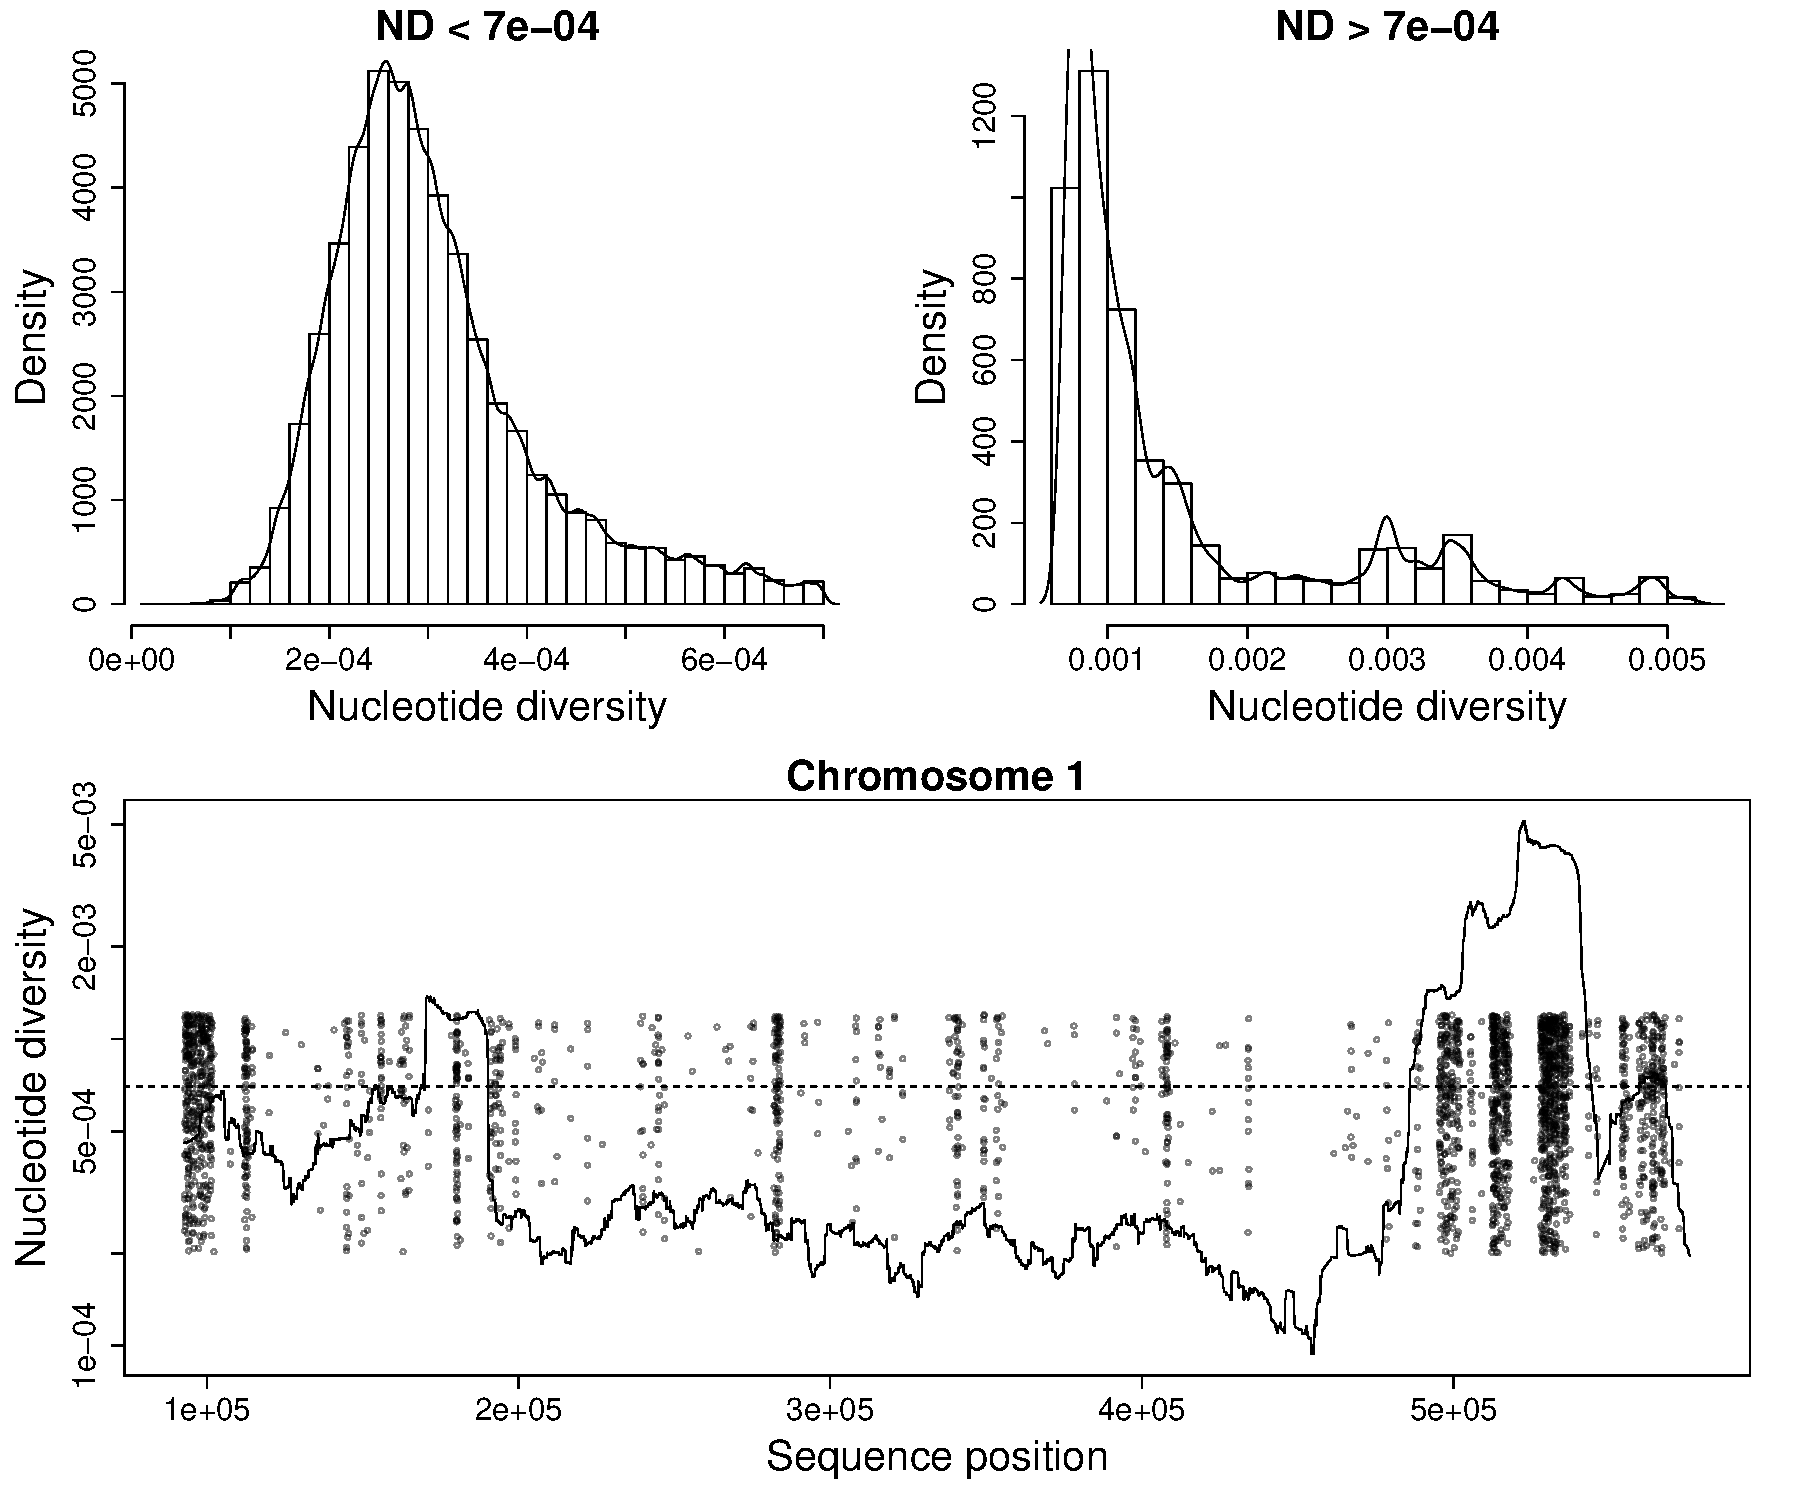
\includegraphics[width=0.7\textwidth]{{supFigures/nd_hist.pdf}}
  \caption{Nucleotide diversity with window size of 20,000. Top two histogram show the heavy tail of ND beyond 0.0007. Bottom figure show ND along {\it P. falciparum} chromosome 1. Scattered Points mark chromosome positions of poorly genotyped SNPs which we exclude from the deconvolution process. These points are jitterred around 0.0007 of visualization.
  }
  \label{fig:nd}
\end{figure}



\subsection{Analysis preparation}
In order to improve the accuracy and efficiency of the deconvolution process, we first split the  data into groups based on genetic similarity. We compute genetic distance between two samples as follows:
\begin{equation}
d(x, y) = \sum_{l}^{L}\textrm{WSAF}_{x,l} * (1-\textrm{WSAF}_{y,l}) + \textrm{WSAF}_{x,l} * (1-\textrm{WSAF}_{y,l})
\end{equation}
where $l$ represents an arbitrary locus, $L$ denotes the total number of loci, and $\textrm{WSAF}_{s,l}$ indicates the non-reference within-sample allele frequency for sample $s$ at locus $l$. $\textrm{WSAF}_{s,l}$ is then given by $\textrm{WSAF}_{s,l} = \frac{a_{s,l}}{r_{s,l}+a_{s,l}}$ where $a_{s,l}$ is the number of read counts supporting the alternative allele in sample $s$ at locus $l$, and $r_{s,l}$ is the number of read counts supporting the reference allele in sample $s$ at locus $l$.

We find that samples from the same geographical region differentiate into clear groups. We use this initial grouping as the basis for defining the reference panels that assist deconvolution. The geographical groups arising from this analysis are listed below. In order to reduce computational time, we restrict to polymorphic sites in each population group:
\begin{enumerate}
  \item Malawi, Congo, with 349,242 sites.
  \item Ghana (Navrongo), with 508,606 sites.
  \item Nigeria, Senegal, Mali, with 210,819 sites.
  \item The Gambia, Guinea, Ghana (Kintampo), with 250,827 sites.
  \item Cambodia (Pursat), Cambodia (Pailin), Thailand (Sisakhet), with 44,317 sites.
  \item Vietnam, Laos, Cambodia (Ratanakiri), Cambodia (Preah Vihear), with 88,410 sites.
  \item Bangladesh, Myanmar, Thailand (Mae Sot), Thailand (Ranong), with 84,868 sites.
\end{enumerate}


%\begin{figure}[htp]
  %\centering{}
  %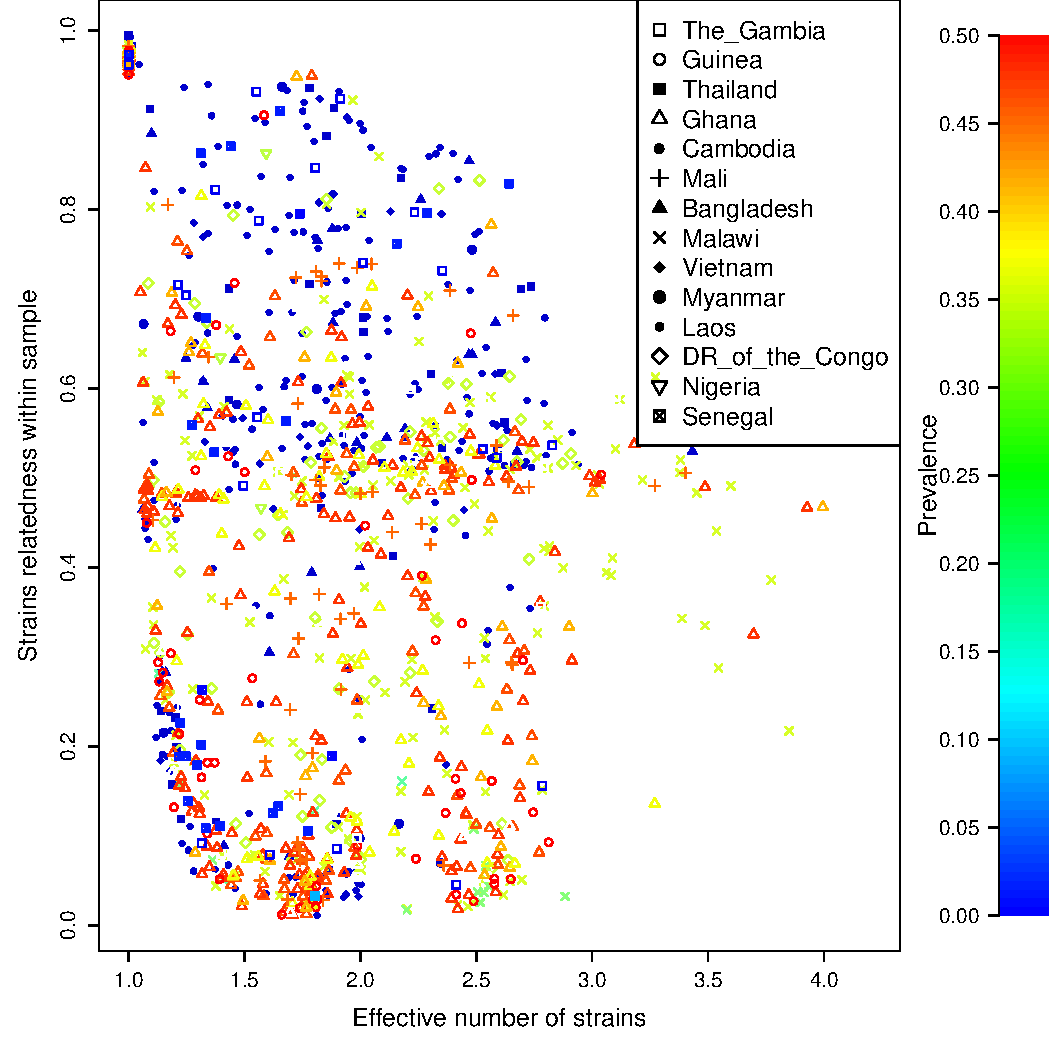
\includegraphics[width=0.8\textwidth]{effK_IBD_colored.pdf}
  %\caption{}\label{fig:tmp1}
%\end{figure}



%\begin{figure}[htp]
  %\centering{}
  %\includegraphics[width=0.8\textwidth]{{llkDiff_vs_eff_k_diff.ibd}.png}
  %\\
  %\includegraphics[width=0.8\textwidth]{{llkDiff_vs_eff_k_diff}.png}
  %\caption{}\label{fig:tmp2}
%\end{figure}


\subsection{Haplotype quality assessment}

We noticed that DEploid-IBD produced chimeric haplotypes when faced with difficult mixtures. For instance, mixed infections in which the co-existing strains have the same relative proportion (e.g. $k=4$ with each strain having a proportion of 25\%), or samples in which proportions are very unbalanced (e.g. k=2 with the marginal strain at 2\%). These artefactual haplotypes show a significant deficit or excess of genetic diversity that cannot be explained in terms of their genetic relationship to the reference genome used for mapping and assembly (3D7). To discard problematic haplotypes, we devised a simple but stringent filtering strategy based on $z$-scores. For each population, we computed the distribution of alternative calls observed within the subset of clonal samples ($k=1$) in a population. Using this distribution as reference, we computed a $z$-score for each haplotype in a population following

$$z_i = \frac{a_i - \bar{a_r}}{\sigma_r},$$ where $a_i$ denotes the number of alternative calls in the haplotype $i$, and $\bar{a}_r$ and $\sigma_r$ are, respectively, the mean and standard deviation of observed alternative calls in the clonal set of samples from the population of origin. We only retain haplotypes with a $z$-score in the range $(-3,3)$, thus discarding any strain that is three or more standard deviations away, in terms of alternative calls, from the mean observed for clonal samples. By using the set of clonal samples as the reference distribution, we approximate the number of alternative calls expected in a genome belonging to that population, which serves as a proxy for genetic diversity but is easier to compute. Supp. Figure \ref{fig:ghana-filtering} shows an example of this filtering process for the most problematic population in the dataset (Ghana). Supp. Table \ref{table:haps-discarded-by-country} lists the number of haplotypes discarded by population while Supp. Table \ref{table:haps-discarded-by-COI} describes the number of haplotypes discarded by COI level.


\begin{figure}[ht]
  \centering
    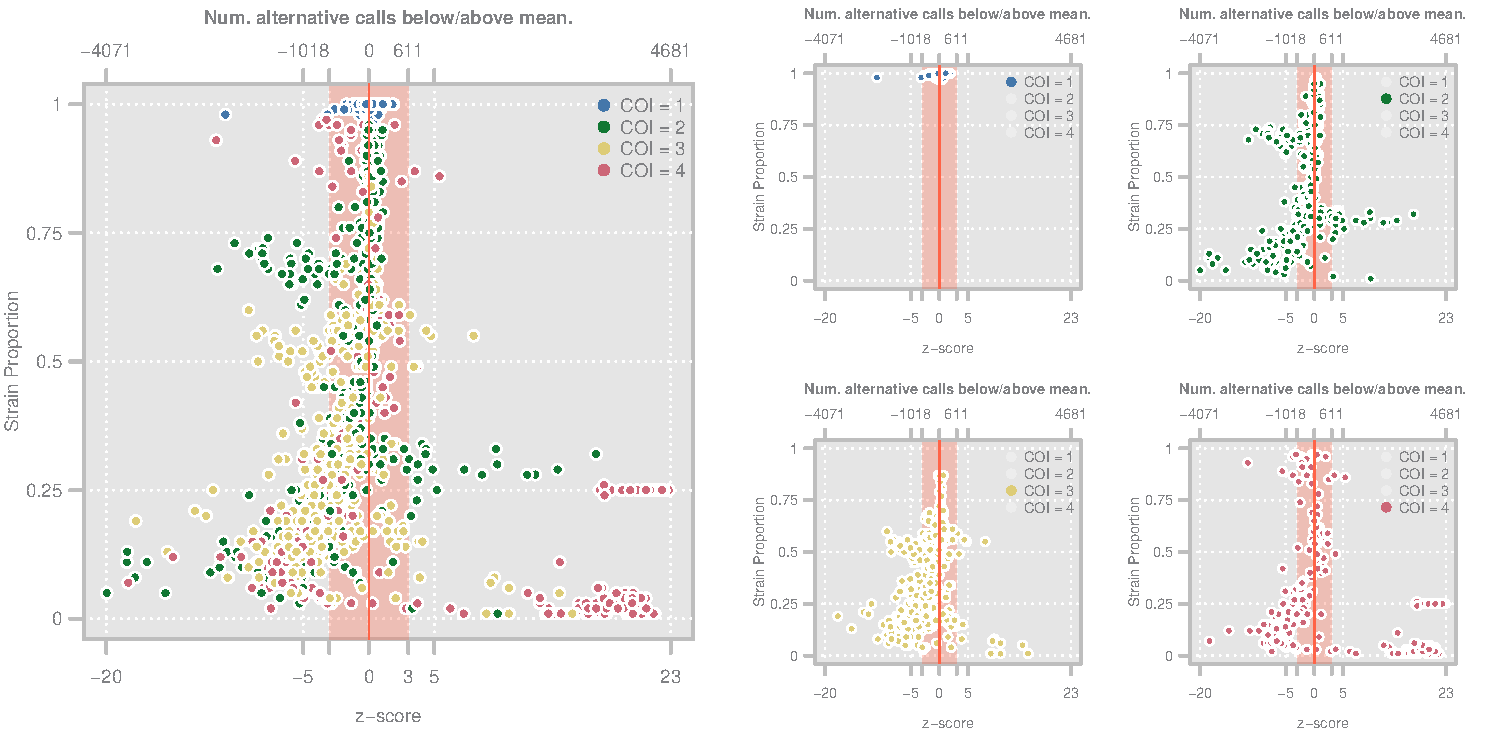
\includegraphics[width=1\textwidth]{figures/qualityGhana.pdf}
  \caption{Diagnostic plots showing the distribution of haplotype quality ($z$-scores) for the Ghanian samples. Left. Scatterplot showing the relationship between haplotype $z$-score and strain proportion. The top axis shows the number of alternative calls below/above the mean of the subset of clonal samples that correspond to a given $z$-score. The vertical red line denotes a $z$-score of $0$ whereas the red-shaded area indicate the haplotypes we retain Point colors show the COI level of the sample. Right. Four views of the same plot in which the samples have been highlighted according to their COI level.}
    \label{fig:ghana-filtering}
\end{figure}



\begin{table}[ht]
\centering
\begin{tabular}{r|r|r|r}
\textbf{Country}  & \textbf{Discarded} & \textbf{Retained} &\textbf{Fraction Discarded} \\
\hline
Bangladesh & 25 & 69 & 0.27 \\
Cambodia & 108 & 697 & 0.13 \\
DR. of Congo & 62 & 155 & 0.29 \\
Ghana & 493 & 609 & 0.45 \\
Guinea & 79 & 88 & 0.47 \\
Laos & 28 & 110 & 0.20 \\
Malawi & 233 & 341 & 0.41 \\
Mali & 37 & 140 & 0.21 \\
Myanmar & 7 & 71 & 0.09 \\
Senegal & 2 & 167 & 0.01\\
Thailand & 28 & 169 & 0.14 \\
The Gambia & 22 & 73 & 0.23 \\
Vietnam & 23 & 113 & 0.17\\
\hline
\textbf{Total} & 1147 & 2802 & 0.29
\end{tabular}
\vspace{.2cm}
\caption{Number of haplotypes discarded and retained for each population in the Pf3k dataset.}
\label{table:haps-discarded-by-country}
\end{table}


\begin{table}[ht]
\centering
\begin{tabular}{r|r|r|r}
\textbf{COI}  & \textbf{Retained} & \textbf{Discarded} & \textbf{Fraction Discarded} \\
\hline
1 & 1331 & 34 & 0.02 \\
2 & 669 & 291 & 0.30 \\
3 & 583 & 533 & 0.48 \\
4 & 219 & 289 & 0.57 \\
\hline
\textbf{Total} & 2802 & 1147 &  \\
\hline
\textbf{Fraction} & 0.71 & 0.29 & \\
\end{tabular}
\vspace{.2cm}
\caption{Number of haplotypes retained and discarded stratified by COI level.}
\label{table:haps-discarded-by-COI}
\end{table}


\subsection{Combining clonal sample pairs for background IBD computation}
We combined randomly selected clonal sample pairs to create artificial mixed infections for  each country, as a way to generate a background IBD distribution. We assume these artifical mixed infections mimic infections generated from two independent mosquito bites. In this setting, strain proportions are determined by their median read depth.  Sample coverage is obtained by accumulating the reference and alternative allele counts of two clonal samples. Similar to {\tt DEploidIBD} deconvolution, high allele count SNPs generated during this process caused high leverage in the model. Additionally, the sample sequence depth and skewness are heterogeneous due to different sample preparation and sequencing protocols. We reduce the {\tt DEploidIBD} filtering threshold from 99.5\% to 80\%, and use low recombination probabilities to avoid false IBD break detections. We validated our method using lab crosses \citep{Miles2016}, and compared the IBD block detections using \citet{Li2003}'s painting with parental strains and {\tt DEploidIBD} algorithm (Figure~\ref{fig:bgibd}).


\begin{figure}[ht]
  \centering{}
  %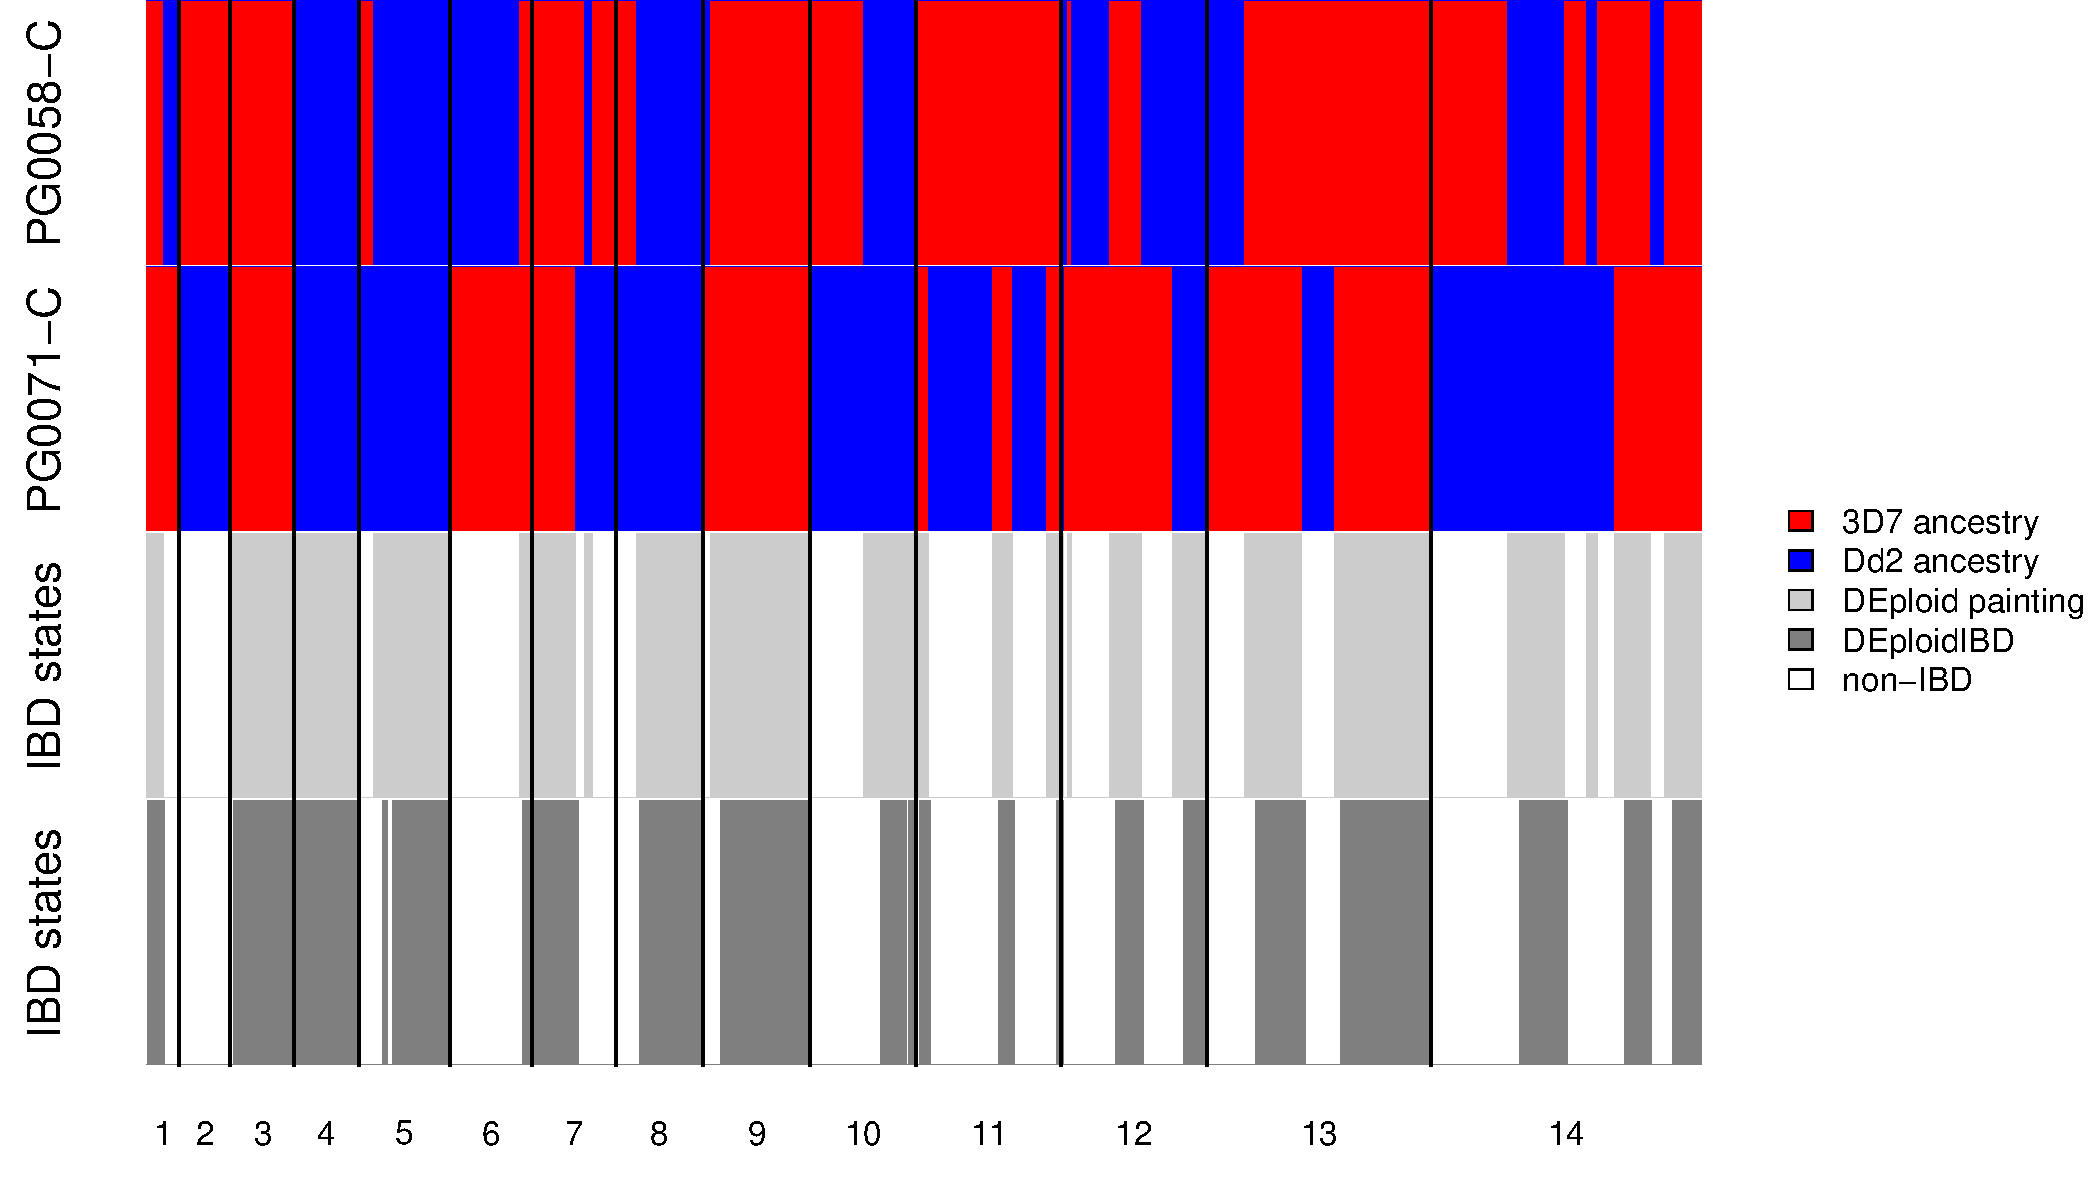
\includegraphics[width = .85\textwidth]{bgIBDvalidation/bgIBD.pdf}
  \subfloat[]{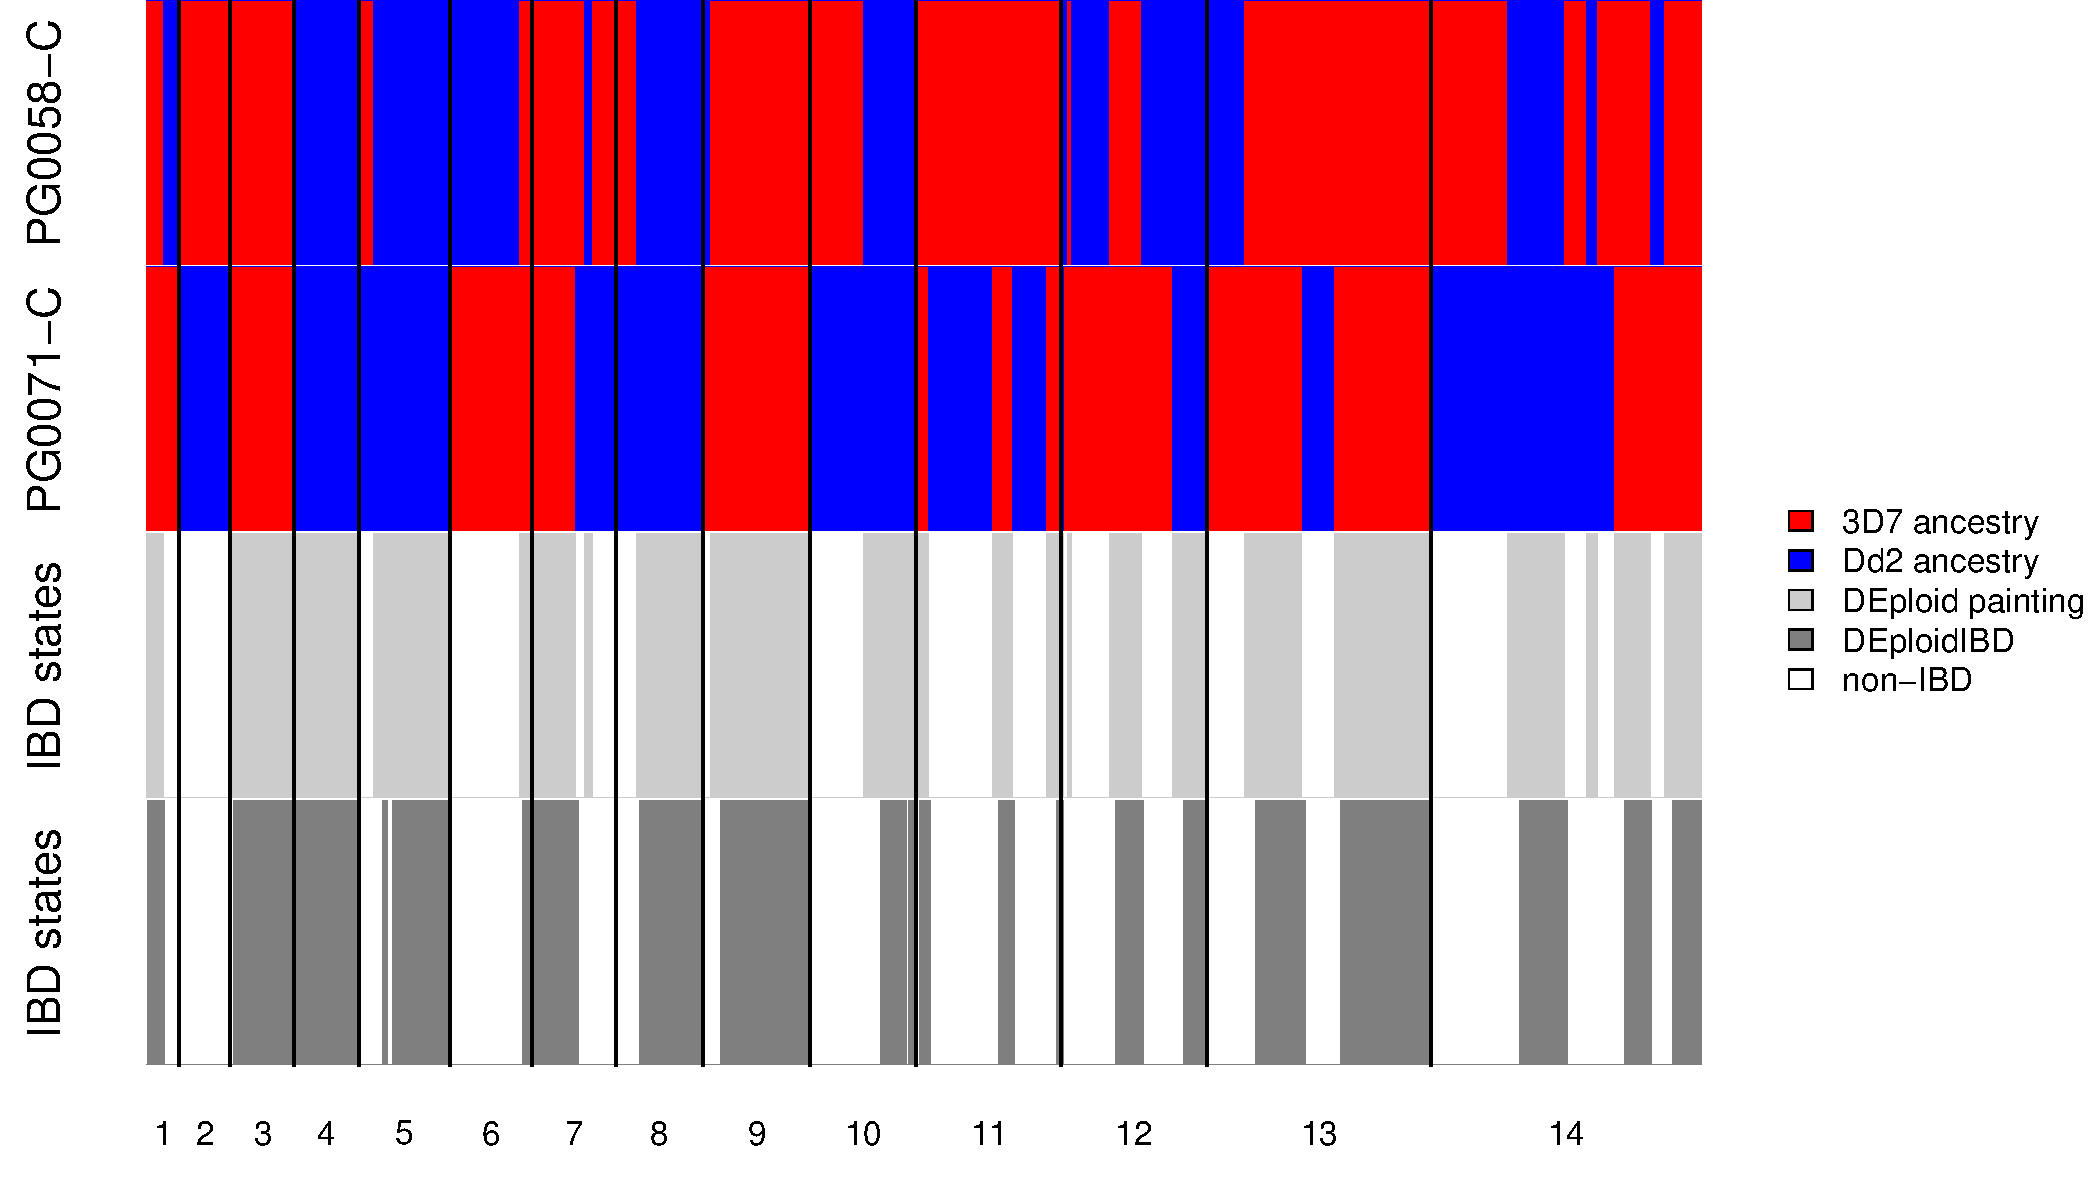
\includegraphics[width = .65\textwidth]{bgIBDvalidation/bgIBD.pdf}}
  \subfloat[]{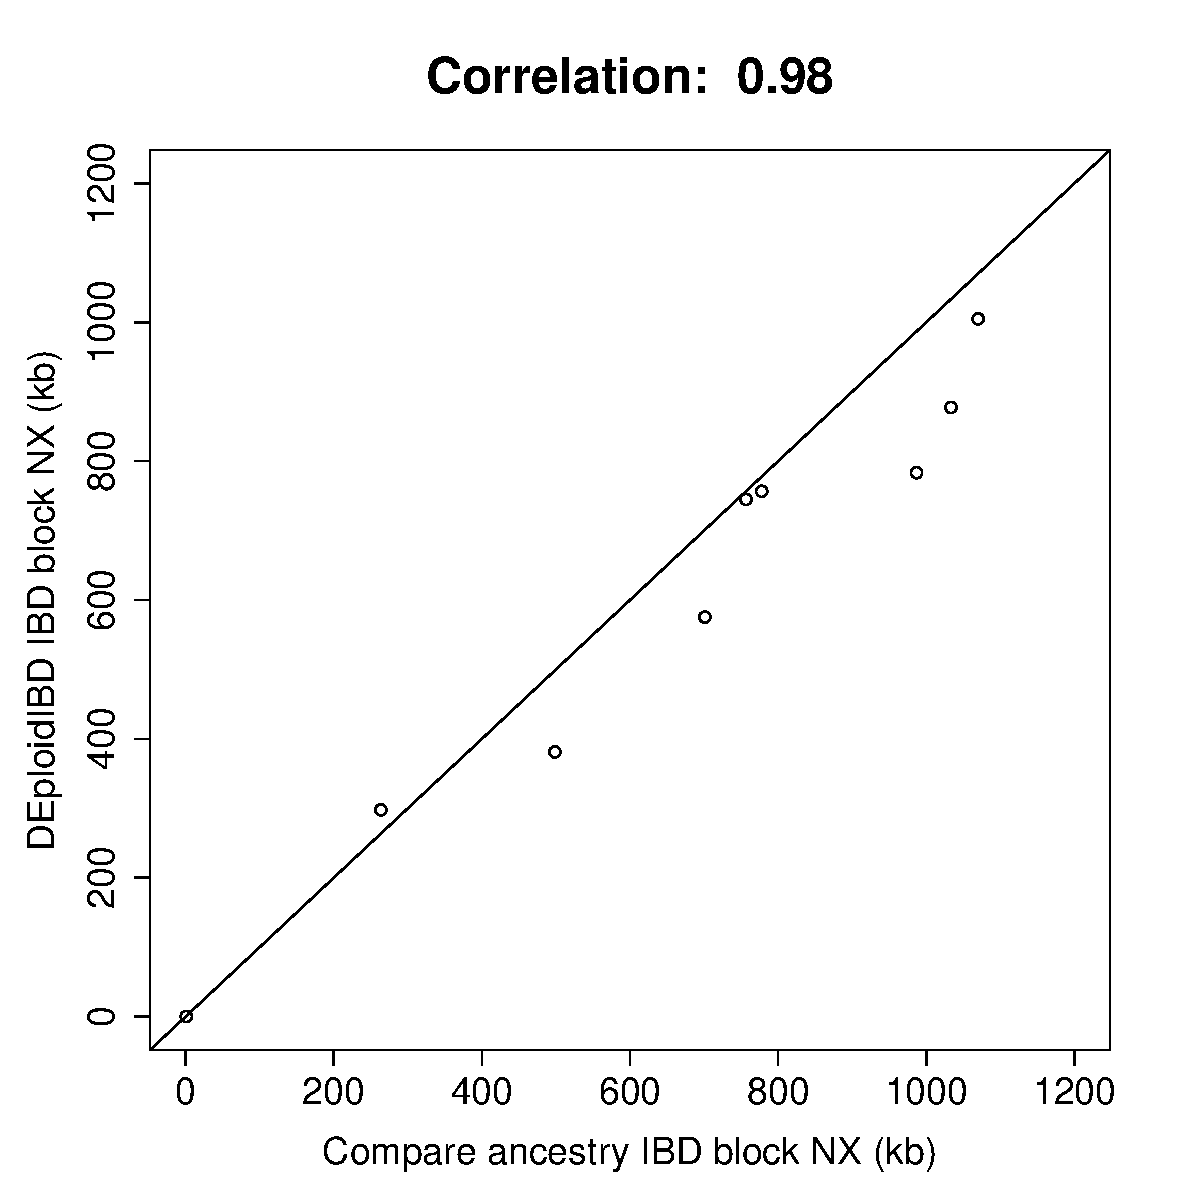
\includegraphics[width = .35\textwidth]{bgIBDvalidation/bgN50.pdf}}
  %\subfloat[]{\includegraphics[width = .85\textwidth]{bgIBDvalidation/IBDtracklengthVsPercentage_data_clean.pdf}}
  \caption{(A) Comparison of IBD block detection of {\tt DEploidIBD} using artificial mixtures of lab crosses PG0071-C and PG0058-C (last track) with IBD block detection from ancestral state inference from \citet{Li2003}. (B) Scatter plot of IBD segment Nx values extracted by comparing clonal sample ancestry and using {\tt DEploidIBD} on artificial mixtures.}\label{fig:bgibd}
\end{figure}

\newpage
\FloatBarrier
\section{Expected levels of IBD in \textit{ P.falciparum } mixed infections}

The amount of IBD observed in a mixed infection is a function of the number of oocysts present in the biting mosquito. We will demonstrate this below.

First, let us briefly review the fundamentals of malaria meiosis. In our case, we imagine a mosquito bites a human host containing two distinct malaria strains. Call these strains $A$ and $B$. Some number of gametocytes of $A$ and $B$ are imbibed during the bite, differentiate into gametes, and undergo fertilization to produce zygotes (reviewed in \citet{Gosh2000}, \citet{Bennink2016}). Some fraction of these zygotes succeed in establishing themselves as oocysts on the mosquito midgut (\citet{Gosh2000}). Three products of fertilization are possible, and thus the oocysts can be either: $A+A$ or $B+B$ (inbred oocysts, $n_{ii}$), or $A+B$ (outbred oocysts, $n_{ij}$). The oocyst state of a mosquito can be characterized by ($n_{ij}$, $n_{ii}$). Which strain is maternal and paternal may vary from oocyst to oocyst, but this is of no consequence here.

A $k=2$ mixed infection is established when two distinct sporozoites, produced from the oocysts of this mosquito, infect a host. Each oocyst produces thousands of sporozoites (\citet{Beir1991}), of four types (discussed in \citet{McKenzie2001}), which pool in the mosquito salivary glands (\citet{Gosh2000}). Imagine drawing a $k=2$ mixed infection from a mosquito harbouring a single outbred oocyst ($n_{ij}$ = 1). In such a mosquito there are two copies of each of the two strains (two sets of sister chromatids; $A$, $A$, $B$, $B$). Thus, ignoring recombination for the present, there are two pairs with an IBD fraction of 1 and, if our original strains are unrelated, the remainder of the ${4 \choose 2}$ pairs will have an IBD of 0. Thus a single $n_{ij}$ oocyst has an expected IBD of $E[\rho]= 2/{4 \choose 2} = 1/3$. We draw pairs without replacement because if sporozoites of only one type seed the infection, it will be $k=1$.  Importantly, neither recombination nor segregation change this result, as they only shuffle how the total identity is distributed between pairs, rather than create or destroy identity (identity is created by DNA replication and destroyed by mutation); the expectation is taken over all pairs and is thus unaffected.

Computing the expected IBD fraction for a mosquito possessing $n_{ij}$ outbred oocysts is an extension of the above. Again ignoring recombination, the expected IBD fraction $E[\rho|n_{ij}]$ is equal to the total number of pairs with an IBD of 1 (IBD pairs), over all possible pairs. In a mosquito with $n_{ij}$ oocysts, we have $2n_{ij}$ copies of each parental strain, thus we have ${2n_{ij} \choose 2}$ IBD pairs for each parental strain, thus $2 {2n_{ij} \choose 2}$ IBD pairs total. Dividing this by the total number of pairs amongst $n_{ij}$ oocysts we have

\begin{equation} \label{eq1}
E[\rho|n_{ij} > 0] = \frac{2{2n_{ij} \choose 2}}{{4n_{ij} \choose 2}} = \frac{2n_{ij} - 1}{4n_{ij} - 1}.
\end{equation}

The above yields $1/3$ for $n_{ij}=1$, approaching $1/2$ as $n_{ij}$ grows. This result has been validated with \texttt{pf-meiosis} in Figure~\ref{fig:validoocyst}.


\begin{figure}[pt]
  \centering{}
  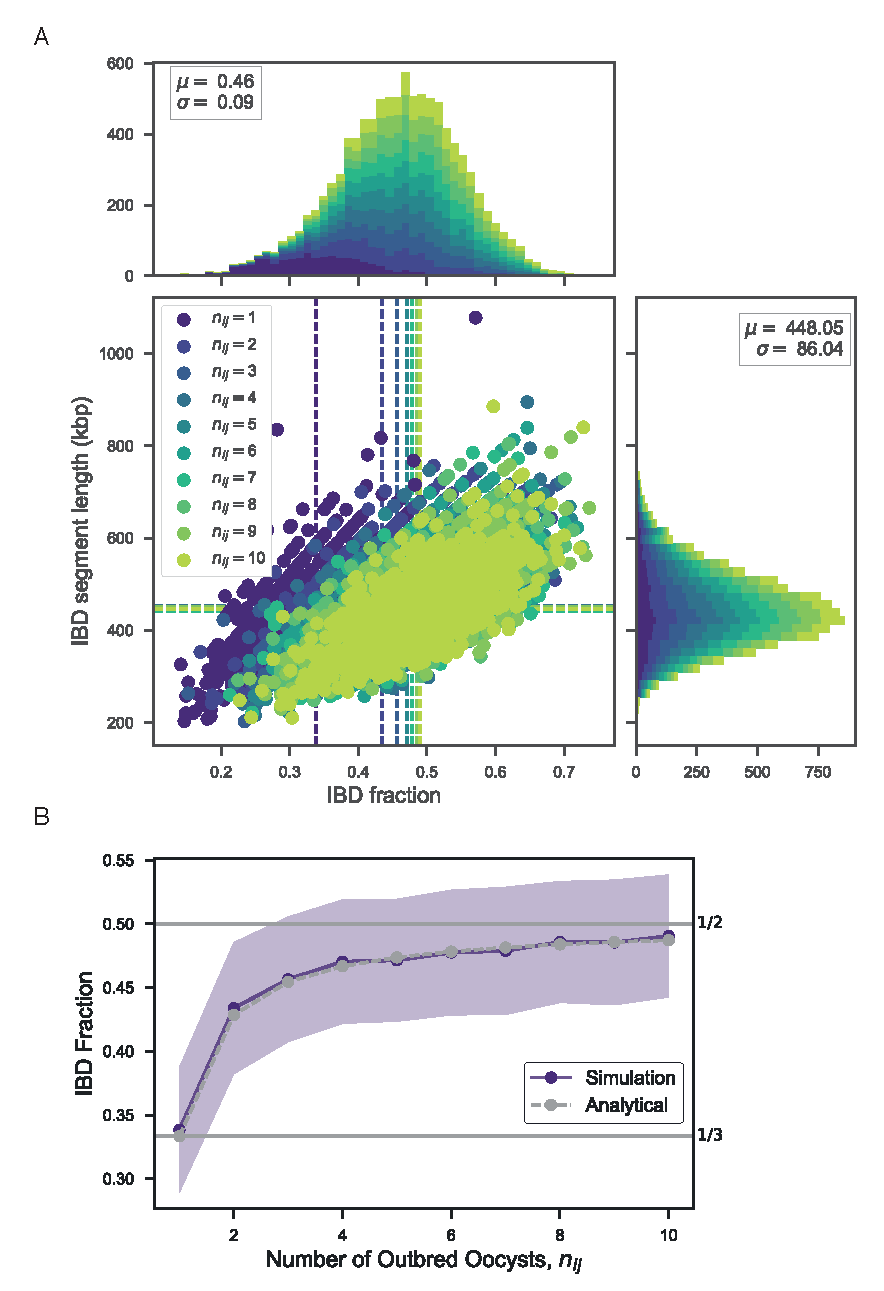
\includegraphics[width = .85\textwidth]{supFigures/supp-Fig1.pdf}
  \caption{Exploring the relationship between number of outbred oocysts ($n_{ij}$) and IBD. (A) Joint IBD fraction and IBD segment length distributions for $k=2$ mixed infections simulated from two unrelated strains and a fixed number of outbred oocysts $n_{ij}$, using \texttt{pf-meiosis}. Mean values for each distribution are indicated by same-color dashed lines. Each distribution is created from 1000 simulated mixed infections. (B) Validation of theoretical result given in text (S1.8). Line plot compares trend in expected IBD fraction with the number of outbred oocysts, $n_{ij}$, for infections simulated in panel A, and analytical expression S1.8.} \label{fig:validoocyst}
\end{figure}

Including $n_{ii}$ oocysts is somewhat involved, as some pairs (selected without replacement) may be identical (thus yielding $k=1$) or completely unrelated (yielding $k=2$, but effectively without having undergone meiosis or producing any detectable recombination breakpoints between parental strains).  We are interested in the expected IBD produced as a result of meiosis between parental strains, and thus for the moment we exclude these pairs. In practice, this means the mosquito must have at least one outbred oocyst, and at least one of the infecting sporozoites must be from an outbred oocyst.

The derivation is as above: first ignoring recombination and segregation, then enumerating all IBD pairs (pairs with IBD fraction of 1) and dividing by the total number of pairs to compute the expectation. Note that the additional IBD pairs possible between an outbred and inbred oocyst are given by the term $8n_{ij}n_{ii}$, and that you can no longer use all possible pairs drawn without replacement as the denominator, but must exclude the pairs described above.

\begin{align}
E[\rho|n_{ij} > 0, n_{ii}] & = \frac{2{2n_{ij} \choose 2} + 8n_{ij}n_{ii}}{2{2n_{ij} \choose 2} + 16n_{ij}n_{ii} + 4n_{ij}^2} \nonumber\\
%& = \frac{{2n_{ij} \choose 2} + 4n_{ij}n_{ii}}{{2n_{ij} \choose 2} + 8n_{ij}n_{ii} + 2n_{ij}^2} \nonumber\\
%& = \frac{n_{ij}(2n_{ij} - 1) + 4n_{ij}n_{ii}}{n_{ij}(2n_{ij} - 1) + 8n_{ij}n_{ii} + 2n_{ij}^2} \nonumber\\
%& = \frac{2n_{ij} - 1 + 4n_{ii}}{2n_{ij} - 1 + 8n_{ii} + 2n_{ij}} \nonumber\\
& = \frac{2(n_{ij} + 2n_{ii}) - 1}{4(n_{ij} + 2n_{ii}) - 1}  \label{eq2}
\end{align}


Which is of a similar form to above, but increases to $1/2$ quicker if more inbred oocysts are present. As before the equation is validated in Figure~\ref{fig:validinbred}A.

\begin{figure}[ht]
  \centering{}
  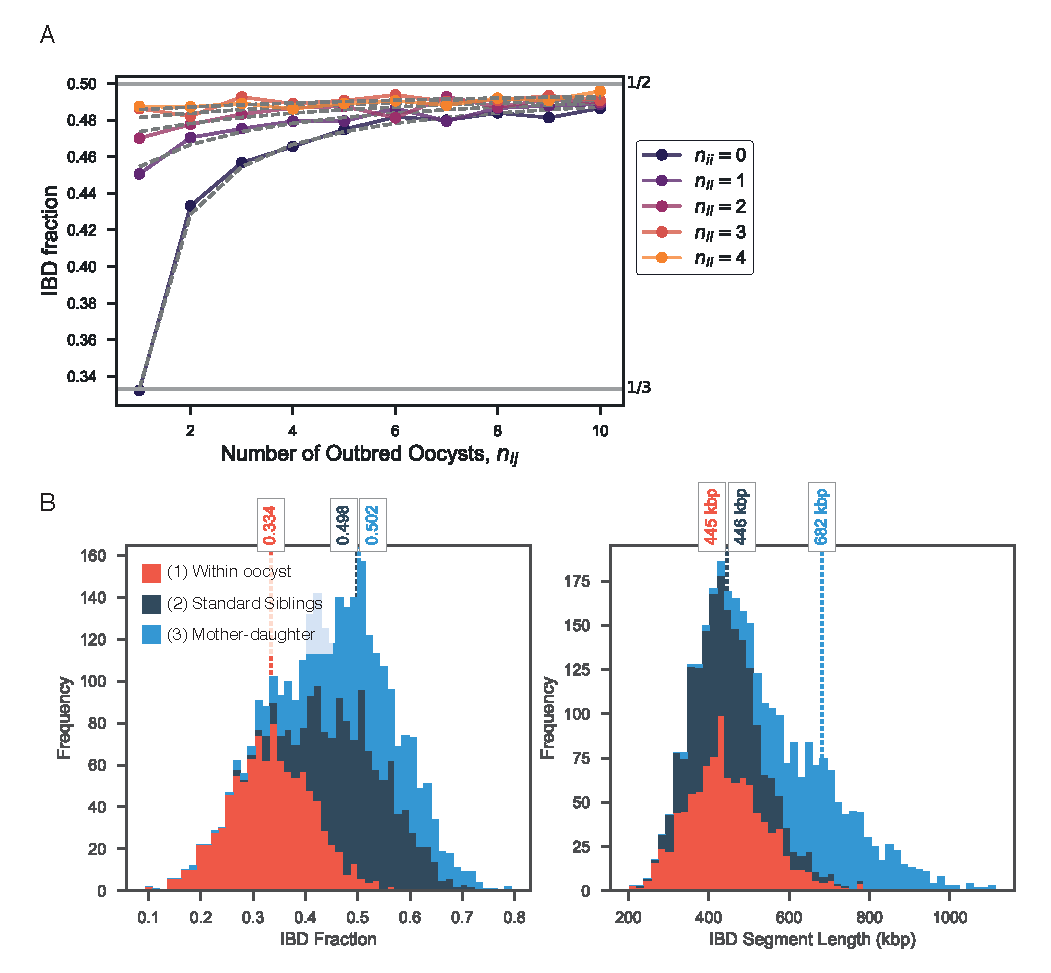
\includegraphics[width = .85\textwidth]{supFigures/supp-Fig2.pdf}
  \caption{Exploring expected IBD allowing for outbred ($n_{ij}$) and inbred ($n_{ii}$) oocysts (A) Validation of expression for expected IBD fraction conditional on outbred $n_{ij}$ and inbred $n_{ii}$ oocysts (S1.9). Line plot compares trend in expected IBD fraction with varying number of outbred (x-axis, $n_{ij}$) and inbred (line color, $n_{ii}$) oocysts and the analytical expression S1.9 (grey dashed lines). (B) Using \texttt{pf-meiosis} to simulate $k=2$ mixed infections generated from (1) two strains from the same outbred oocyst from ($n^{o=1}_{ij}$, 'Within oocyst'); (2) two strains different outbred oocysts($n^{o=2}_{ij}$, 'Standard Siblings'); (3) one strain from an outbred and one strain from an inbred oocyst ($n^{o=2}_{ij, ii}$, 'Mother-daughter').} \label{fig:validinbred}
\end{figure}

The expression for $E[\rho|n_{ij} > 0, n_{ii}]$ can also be derived by recognizing that there are three \textit{types} of pairs possible in a mosquito with a collection of $n_{ij}$ and $n_{ii}$ oocysts: (1) a pair can contain two strains from a single $n_{ij}$, ($n^{o=1}_{ij}$); (2) a pair can contain two strains from two different $n_{ij}$, ($n^{o=2}_{ij}$); or (3) a pair can contain one strain from an $n_{ij}$ oocyst and one from an $n_{ii}$ oocyst, $n^{o=2}_{ij, ii}$. Pair type (1) is unique to malaria and has an  $E[\rho|n^{o=1}_{ij}]=1/3$, as shown above; pair type (2) are standard siblings with $E[\rho|n^{o=2}_{ij}]=1/2$; and pair type (3) represent a mother-daughter relationship, also with $E[\rho|n^{o=2}_{ij, ii}]=1/2$. The full IBD fraction and IBD segment length distributions of these pairs were generated using \texttt{pf-meiosis} and can be seen in Figure~\ref{fig:validinbred}B. We enumerate the number of each pair type given $n_{ij}$ and $n_{ii}$, weighted by their expectation, to derive $E[\rho|n_{ij} > 0, n_{ii}]$:


\begin{align}
E[\rho|n_{ij} > 0, n_{ii}] & = \frac{n^{o=1}_{ij}E[f|n^{o=1}_{ij}] + n^{o=2}_{ij}E[f|n^{o=2}_{ij}]
+ n^{o=2}_{ij, ii}E[f|n^{o=2}_{ij, ii}]}{n^{o=1}_{ij} + n^{o=2}_{ij} + n^{o=2}_{ij, ii}} \nonumber\\
& = \frac{ n_{ij}{4\choose 2}1/3 + 16{n_{ij}\choose 2}1/2 + 16n_{ij}n_{ii}1/2}{
n_{ij}{4\choose 2} + 16{n_{ij}\choose 2} + 16n_{ij}n_{ii}} \nonumber\\
%& = \frac{2n_{ij} + 4n_{ij}(n_{ij} - 1) + 8n_{ij}n_{ii}}{6n_{ij} + 8n_{ij}(n_{ij} - 1) + 16n_{ij}n_{ii}}\nonumber\\
%& = \frac{1 + 2(n_{ij} - 1) + 4n_{ii}}{3 + 4(n_{ij} - 1) + 8n_{ii}} \nonumber\\
& = \frac{2(n_{ij} + 2n_{ii}) - 1}{4(n_{ij} + 2n_{ii}) - 1}
\end{align}
As above.

\FloatBarrier
\bibliographystyle{chicagoa}
\bibliography{mixedIBD.bib}

\newpage
\renewcommand{\thepage}{S2--\arabic{page}}
\setcounter{page}{1}

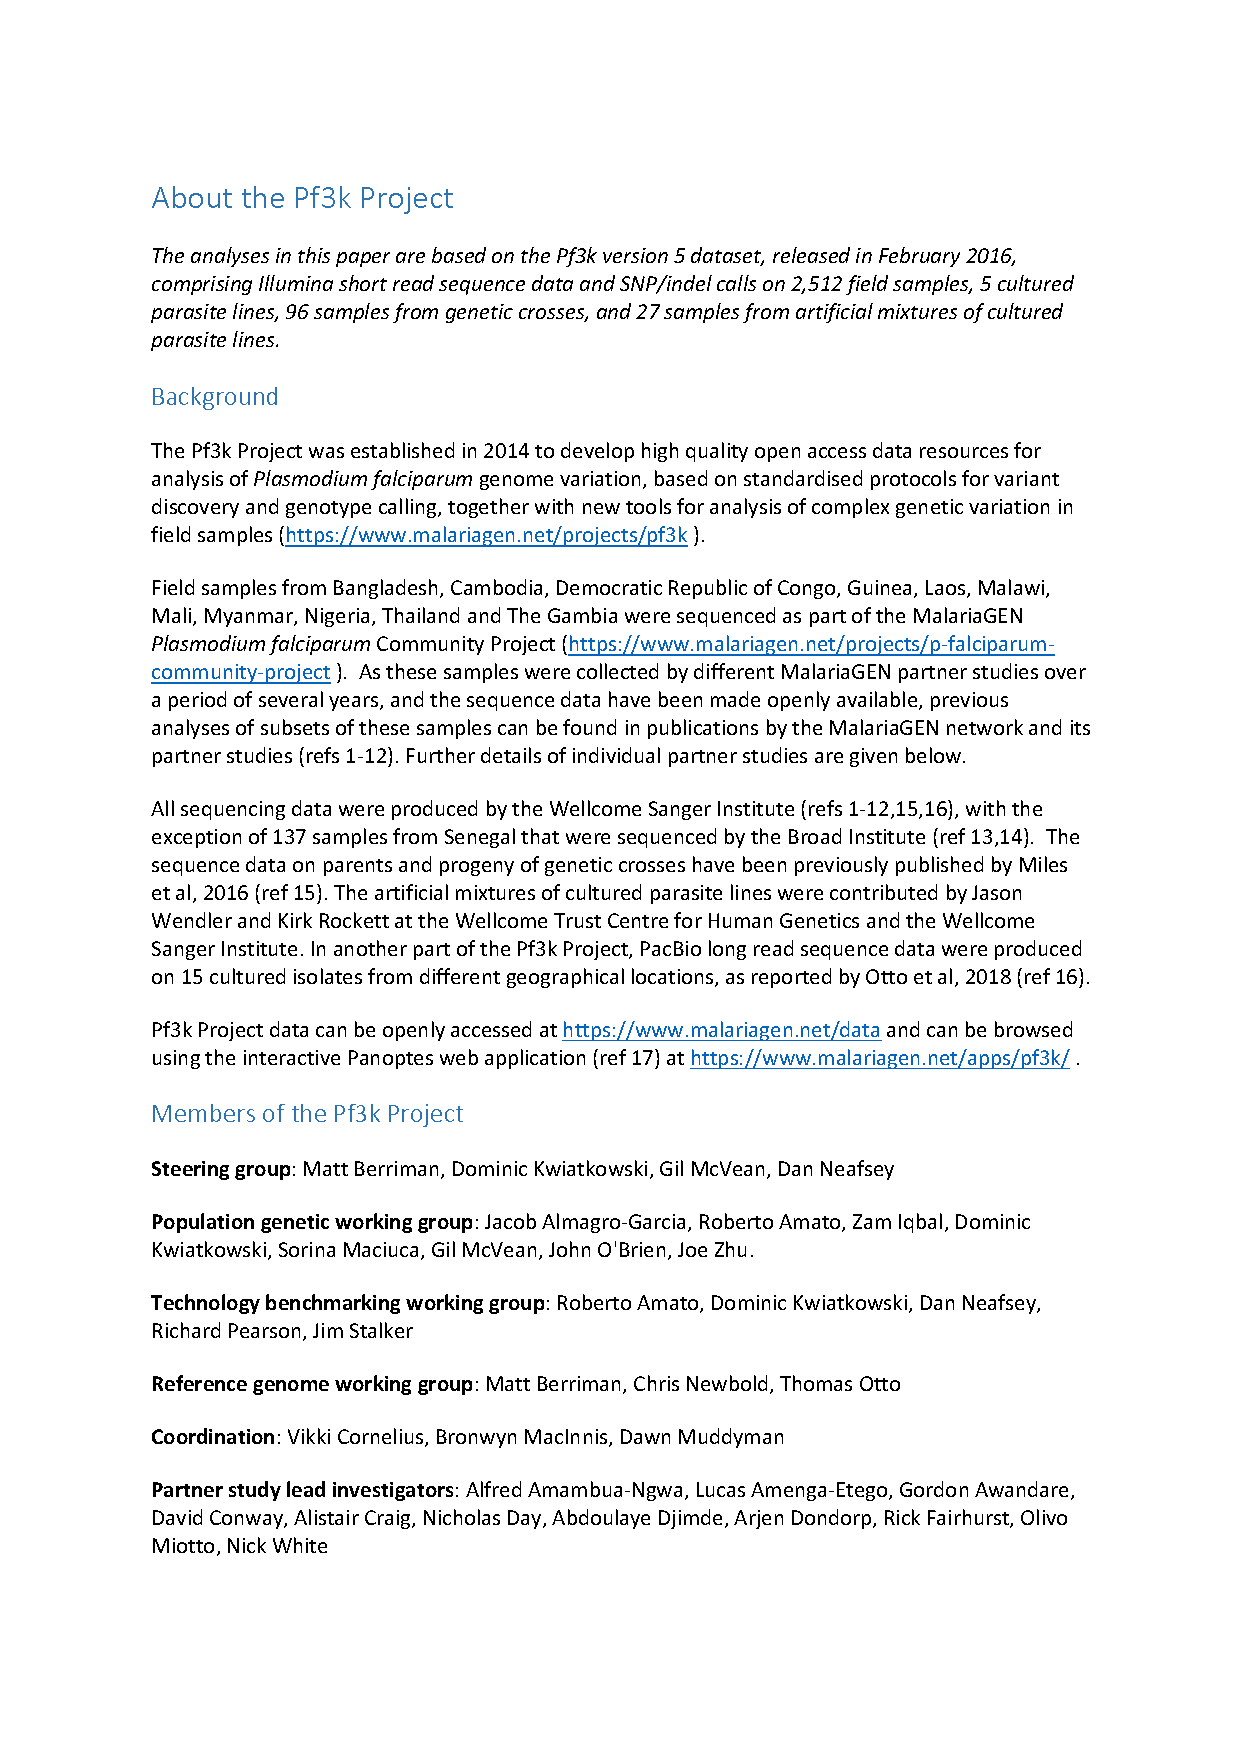
\includepdf[pages=-]{180803_Pf3k_project_info.pdf}

\end{document}
